\subsection{Budowa manipulatora}
\begin{figure}[H]
	\centering
	\resizebox{130mm}{!}{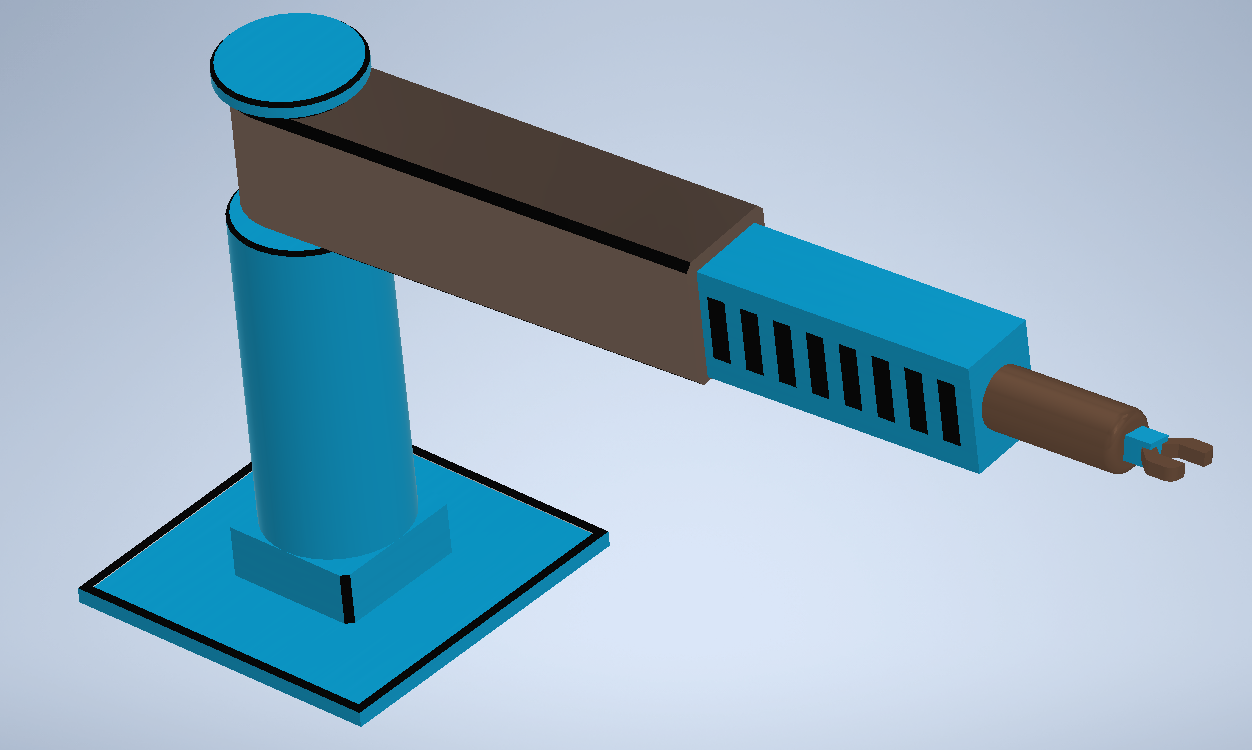
\includegraphics{src/calosc.png}}
	\caption{Projekt manipulatora} 
\end{figure}
Manipulator został zaprojektowany w programie Inventor. Jego konfiguracja to RPR $|--$.


Podczas konstrukcji robota uwzględniliśmy mechaniczne aspekty konstrukcji takie jak:
\begin{itemize}
	\item ograniczenie stopni swobody
	\item zabezpieczenia mechaniczne
\end{itemize}

\begin{figure}[H]
	\centering
	\resizebox{130mm}{!}{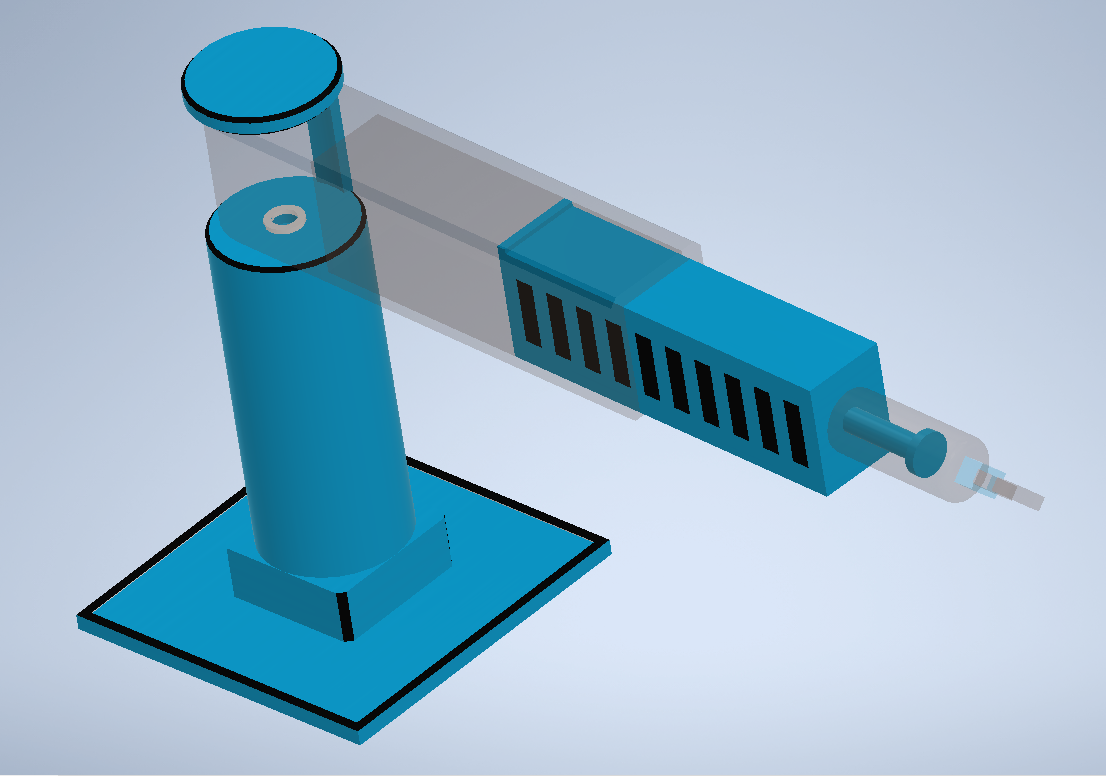
\includegraphics{src/mechanika.png}}
	\caption{Konstrukcja mechaniczna manipulatora} 
\end{figure}
Robot posiada ograniczenia w pierwszych dwóch przegubach
\begin{itemize}
	\item Maksymalne wychylenie kąta $\theta_1$ wynosi 195°
	\item Maksymalne wysunięcie długości $d_1$ wynosi 38cm
\end{itemize}
Ostatni przegub jest zaprojektowany na pełen obrót 360°.


Do pierwszego przegubu zostały dodane podkładki, mające na celu polepszenie stabilności obrotu ramienia robota.


\begin{figure}[H]
	\centering
	\resizebox{130mm}{!}{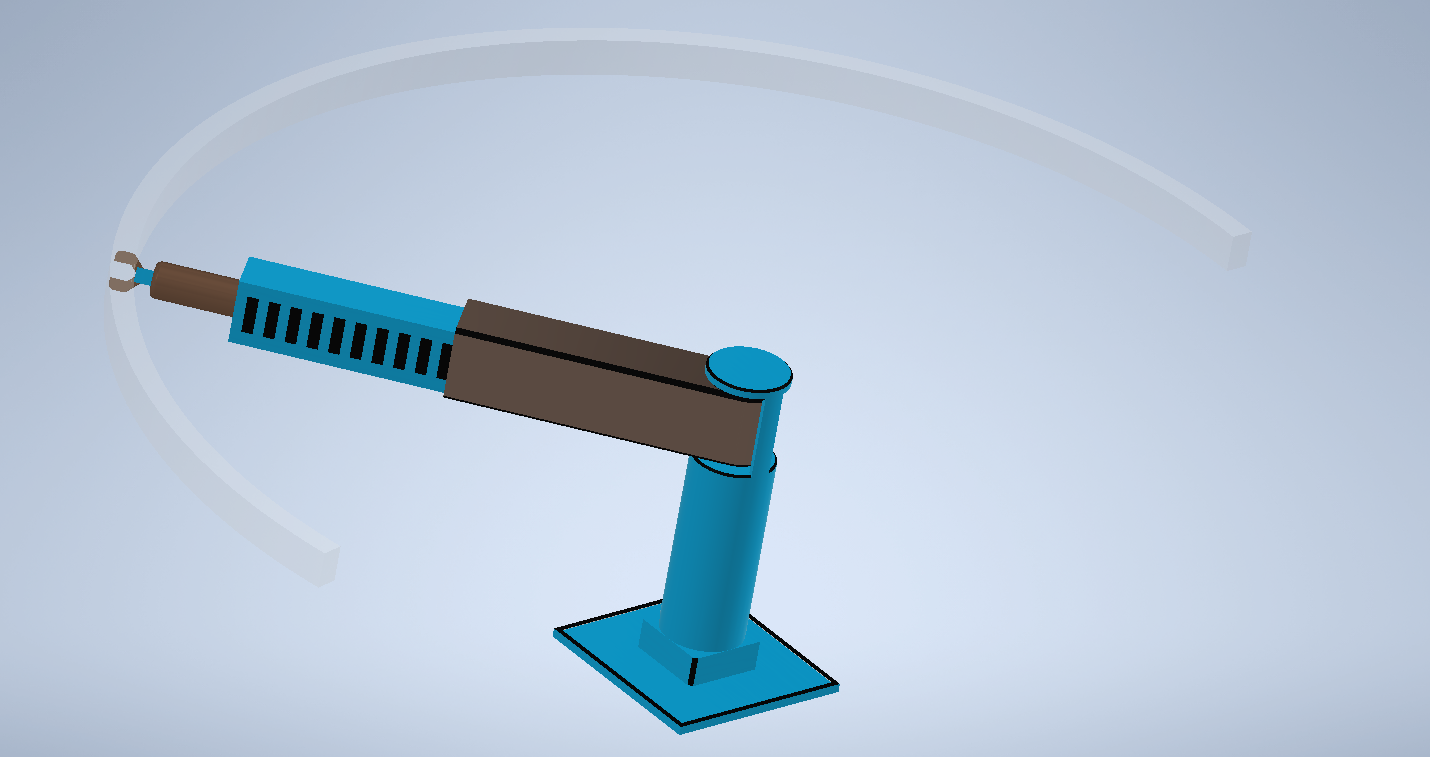
\includegraphics{src/przestrzen_robocza.png}}
	\caption{Przestrzeń robocza manipulatora} 
\end{figure}

 W naszym modelu wybraliśmy ułożenie końcówki TCP równolegle z ostatnim przegubem przesuwnym. Oznacza to, że ten przegub nie odpowiada za pozycje końcówki, a za jej orientację. W związku z tym nasz manipulator może zostać zaprojektowany np. do przykręcania śrub.
 
 \begin{figure}[H]
	\centering
	\resizebox{130mm}{!}{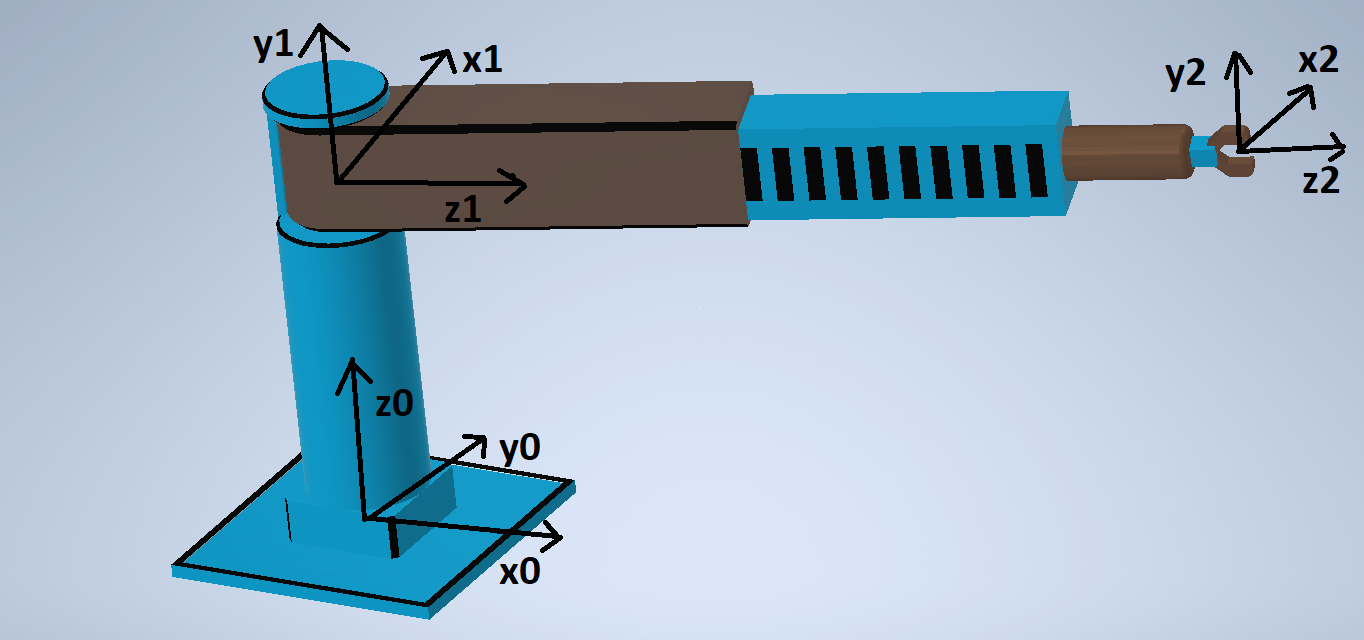
\includegraphics{src/uklad_wspolrzednych.png}}
	\caption{Układy współrzędnych w przegubach manipulatora} 
\end{figure}

\subsection{Program w języku Python}

Do zamodelowania robota skorzystaliśmy z biblioteki RoboticToolBox. Kod znajduje się w funkcji projekt() oraz składa się z trzech etapów:
\begin{enumerate}
    \item inicjacji zmiennych, utworzeniu robota oraz pokazaniu go na interaktywnym wykresie
    \item obliczeniu kinematyki prostej
    \item obliczeniu kinematyki prędkości
\end{enumerate}


\begin{lstlisting}[language=Python]
import roboticstoolbox as rtb
from spatialmath.base.symbolic import *
from roboticstoolbox.tools.trajectory import *


def projekt():

    #inicjacja

    l1=0.4925
    l2=0.5
    alpha1=np.pi/2
    offset1=np.pi/2
    theta1_min=0
    theta1_max=195/360*2*np.pi
    d2_min=0
    d2_max=0.38
    l3=0.221314
    theta3_min=0
    theta3_max= 2 * np.pi

    q_tmp = [symbol('theta1'), symbol('theta2'), symbol('theta3')]

    '''
    #obliczenia na symbolach
    
    robot=rtb.DHRobot(
    [
        rtb.RevoluteDH(d=symbol('l1'), alpha=pi()/2
        , offset=pi()/2),
        rtb.PrismaticDH(offset=symbol('l2')),
        rtb.RevoluteDH(d=symbol('l3'))
    ], name="RPR")
    
    '''

    robot=rtb.DHRobot(
        [
            rtb.RevoluteDH(d=l1, alpha=alpha1, offset=offset1, 
            qlim=[theta1_min, theta1_max]),
            rtb.PrismaticDH(offset=l2, qlim=[d2_min,d2_max]),
            rtb.RevoluteDH(qlim=[theta3_min, theta3_max], d=l3),
        ], name="RPR")

    print(robot)
    robot.teach(robot.q)

    #kinematyka prosta

    T=robot.fkine(q_tmp)
    print(T)

    #kinematyka predkosci
    J=simplify(robot.jacob0(q_tmp))
    print(J)

    #kinematyka odwrotna - na kartce
    #dynamika - na kartce

if __name__ == '__main__':
    projekt()

\end{lstlisting}

\begin{figure}[H]
	\centering
	\resizebox{130mm}{!}{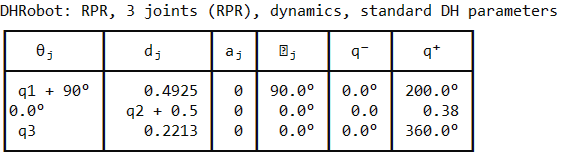
\includegraphics{src/dh.png}}
	\caption{Tablica DH z konsoli programu w języku Python} 
\end{figure}

\begin{figure}[H]
	\centering
	\resizebox{130mm}{!}{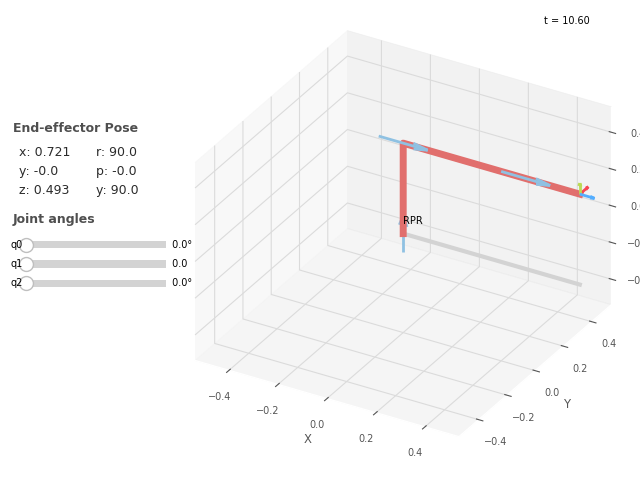
\includegraphics{src/Robotics_Toolbox_for_Python_(Figure_1).png}}
	\caption{Interaktywny układ robota dla programu w języku Python} 
\end{figure}